\documentclass[a4paper]{article}
\usepackage[colorlinks=true,allcolors=blue]{hyperref}
\usepackage{amsmath}
\usepackage{graphicx}
\usepackage{amsfonts}
\usepackage[none]{hyphenat} %this is not necessary for the students to figure out, but a good thing to know
% it also sometimes gets rid of the overfull/underfull box warning



\title{Images exercise}
\author{Me, myself and I}
\date{\today}

\begin{document}


\maketitle

\section*{Images}

Go to \href{https://commons.wikimedia.org/wiki/Commons:Picture_of_the_day#/media/File:Adelie_penguins_in_the_South_Shetland_Islands.jpg}{this link} on Wikimedia Commons and download the picture (to save space, don't download the original file, but the preview). Then insert it here, as shown below.
\begin{figure}[h!]
    \centering
    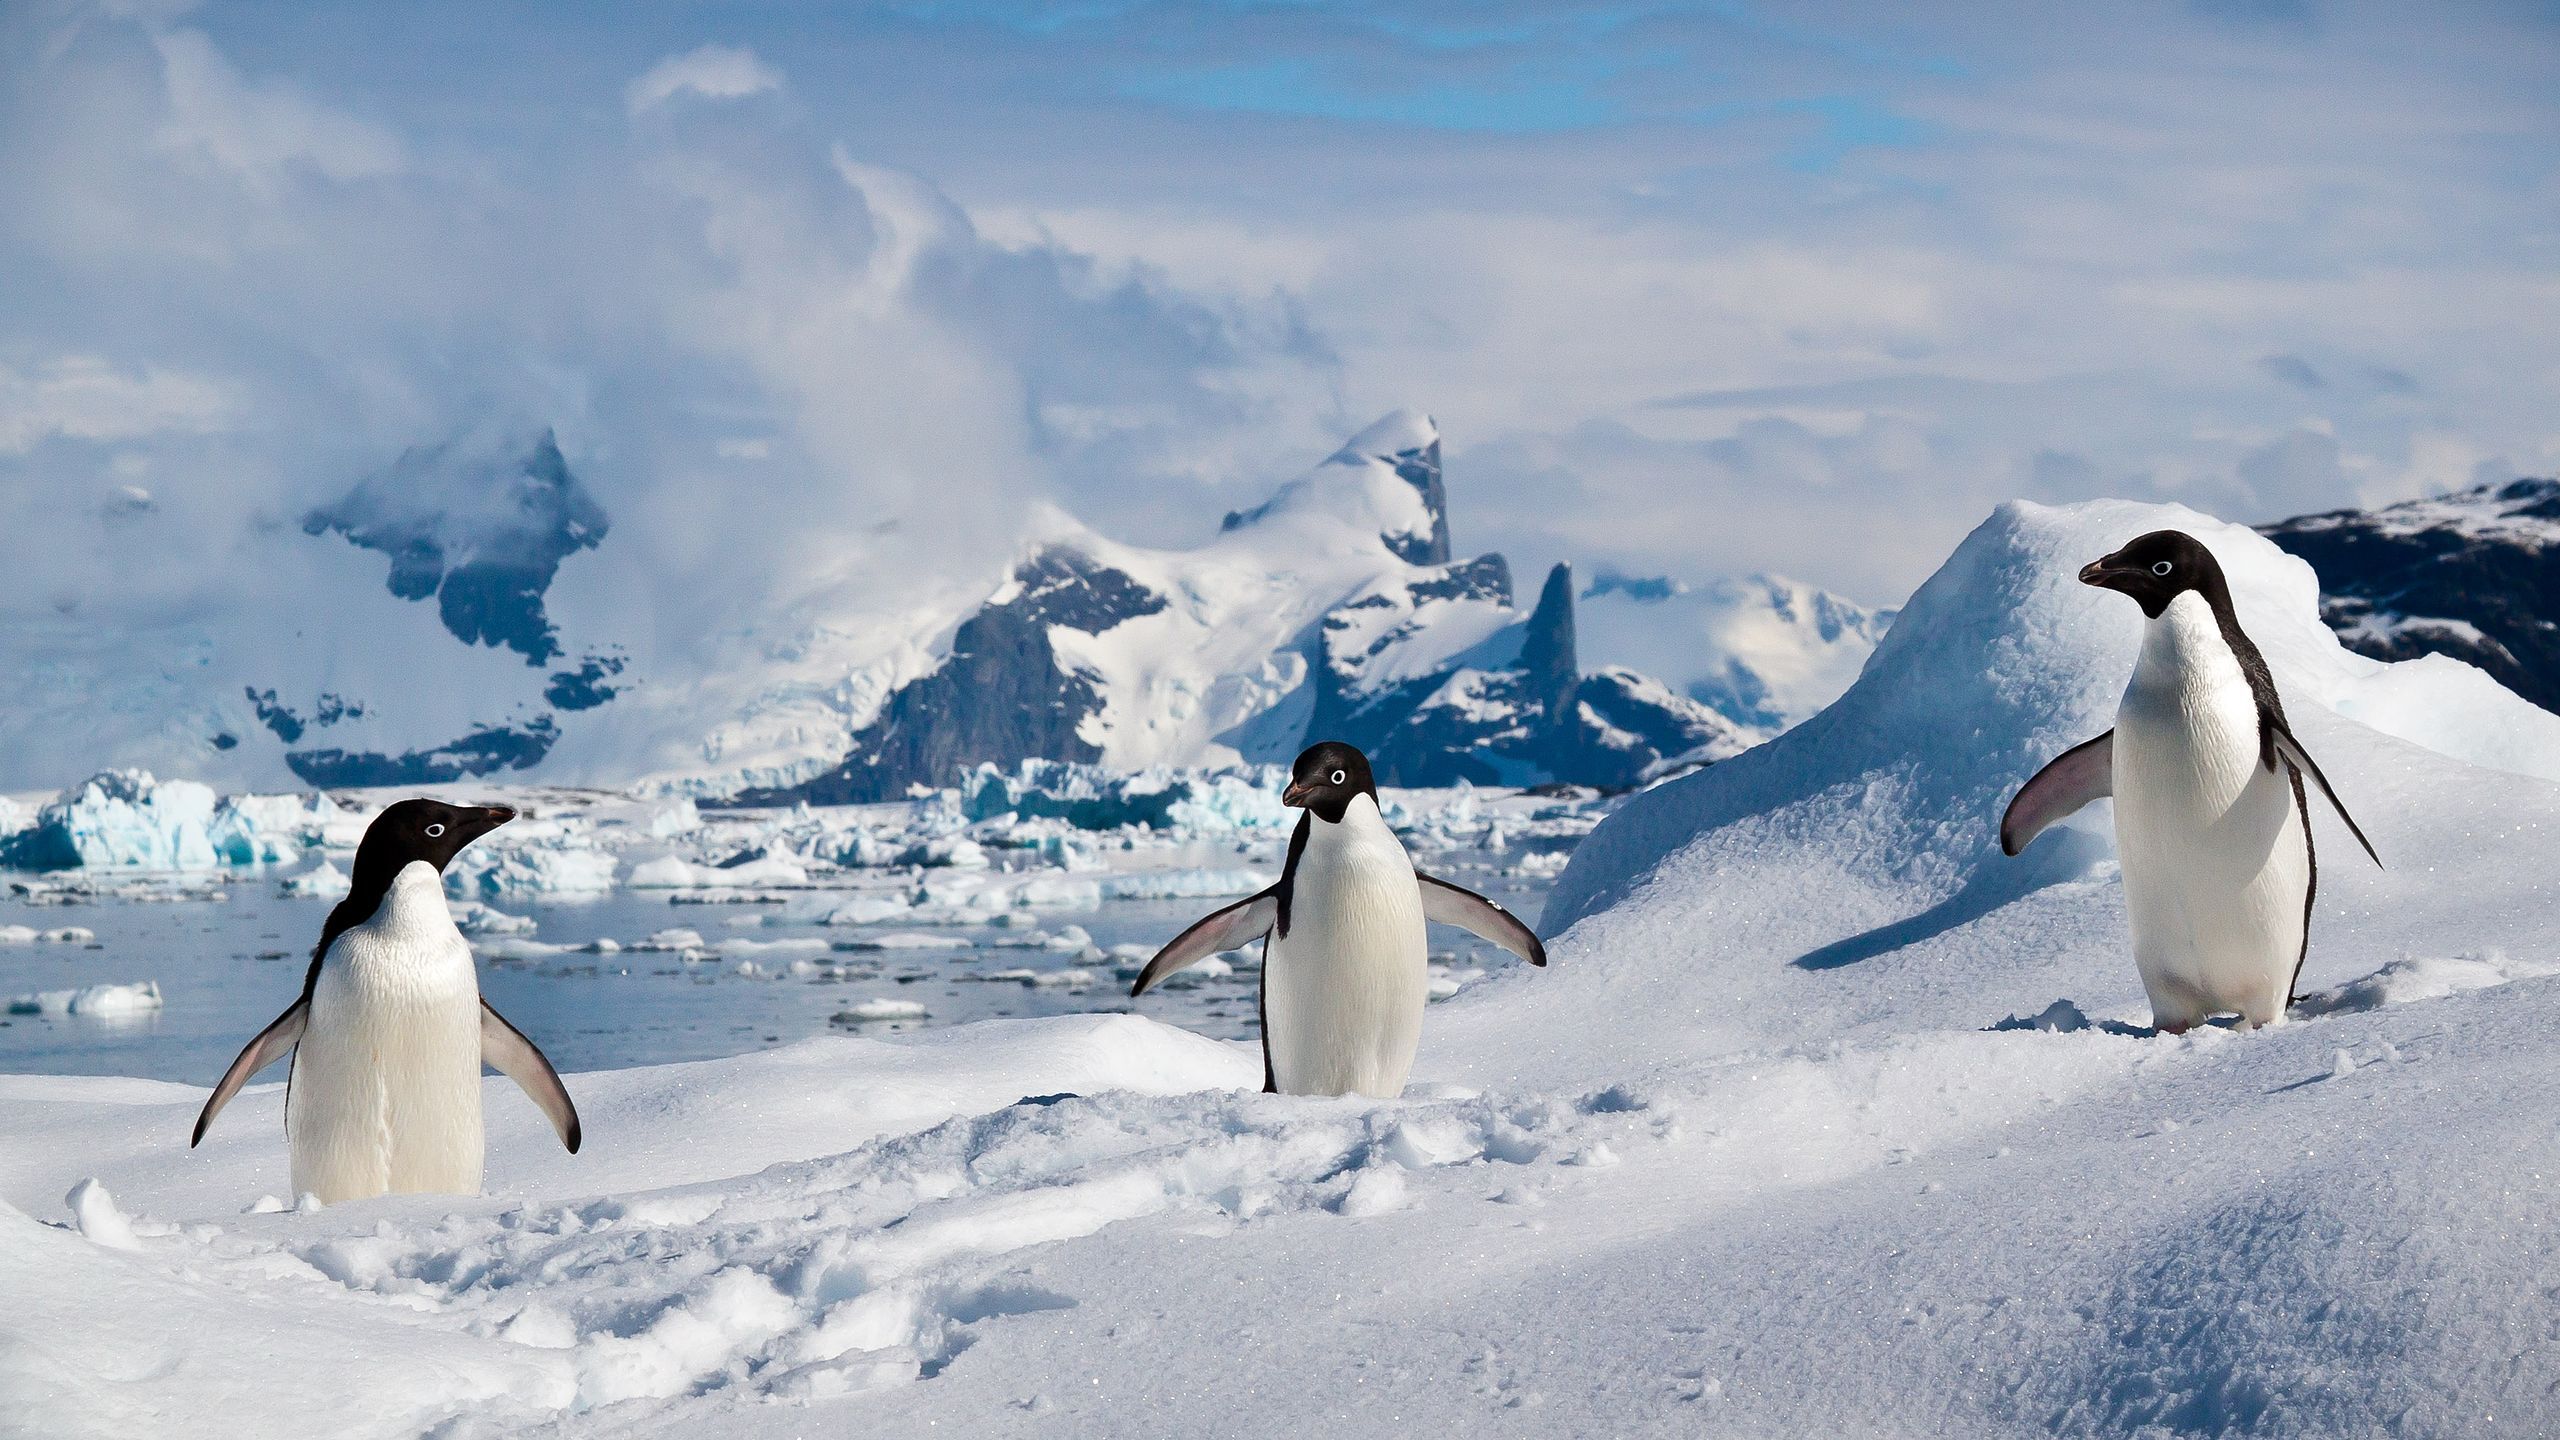
\includegraphics[width=\textwidth]{Adelie_penguins_in_the_South_Shetland_Islands.jpg}
    \caption{Source: \href{https://commons.wikimedia.org/wiki/File:21-224-5054_NNP_Synevyr_RB_18.jpg}{Wikimedia Commons}}
    \label{fig:adelie_penguins}
\end{figure}

Figure \ref{fig:adelie_penguins} shows Adelie penguins in the South Shetland Islands.

\newpage

Now scale it down to 10\% of its size (mind the placement!) and reference it like so: figure \ref{fig:adelie_penguins_scaled} shows the same picture as before, but scaled to 10\% of its size.

\begin{figure}[b!]
    \centering
    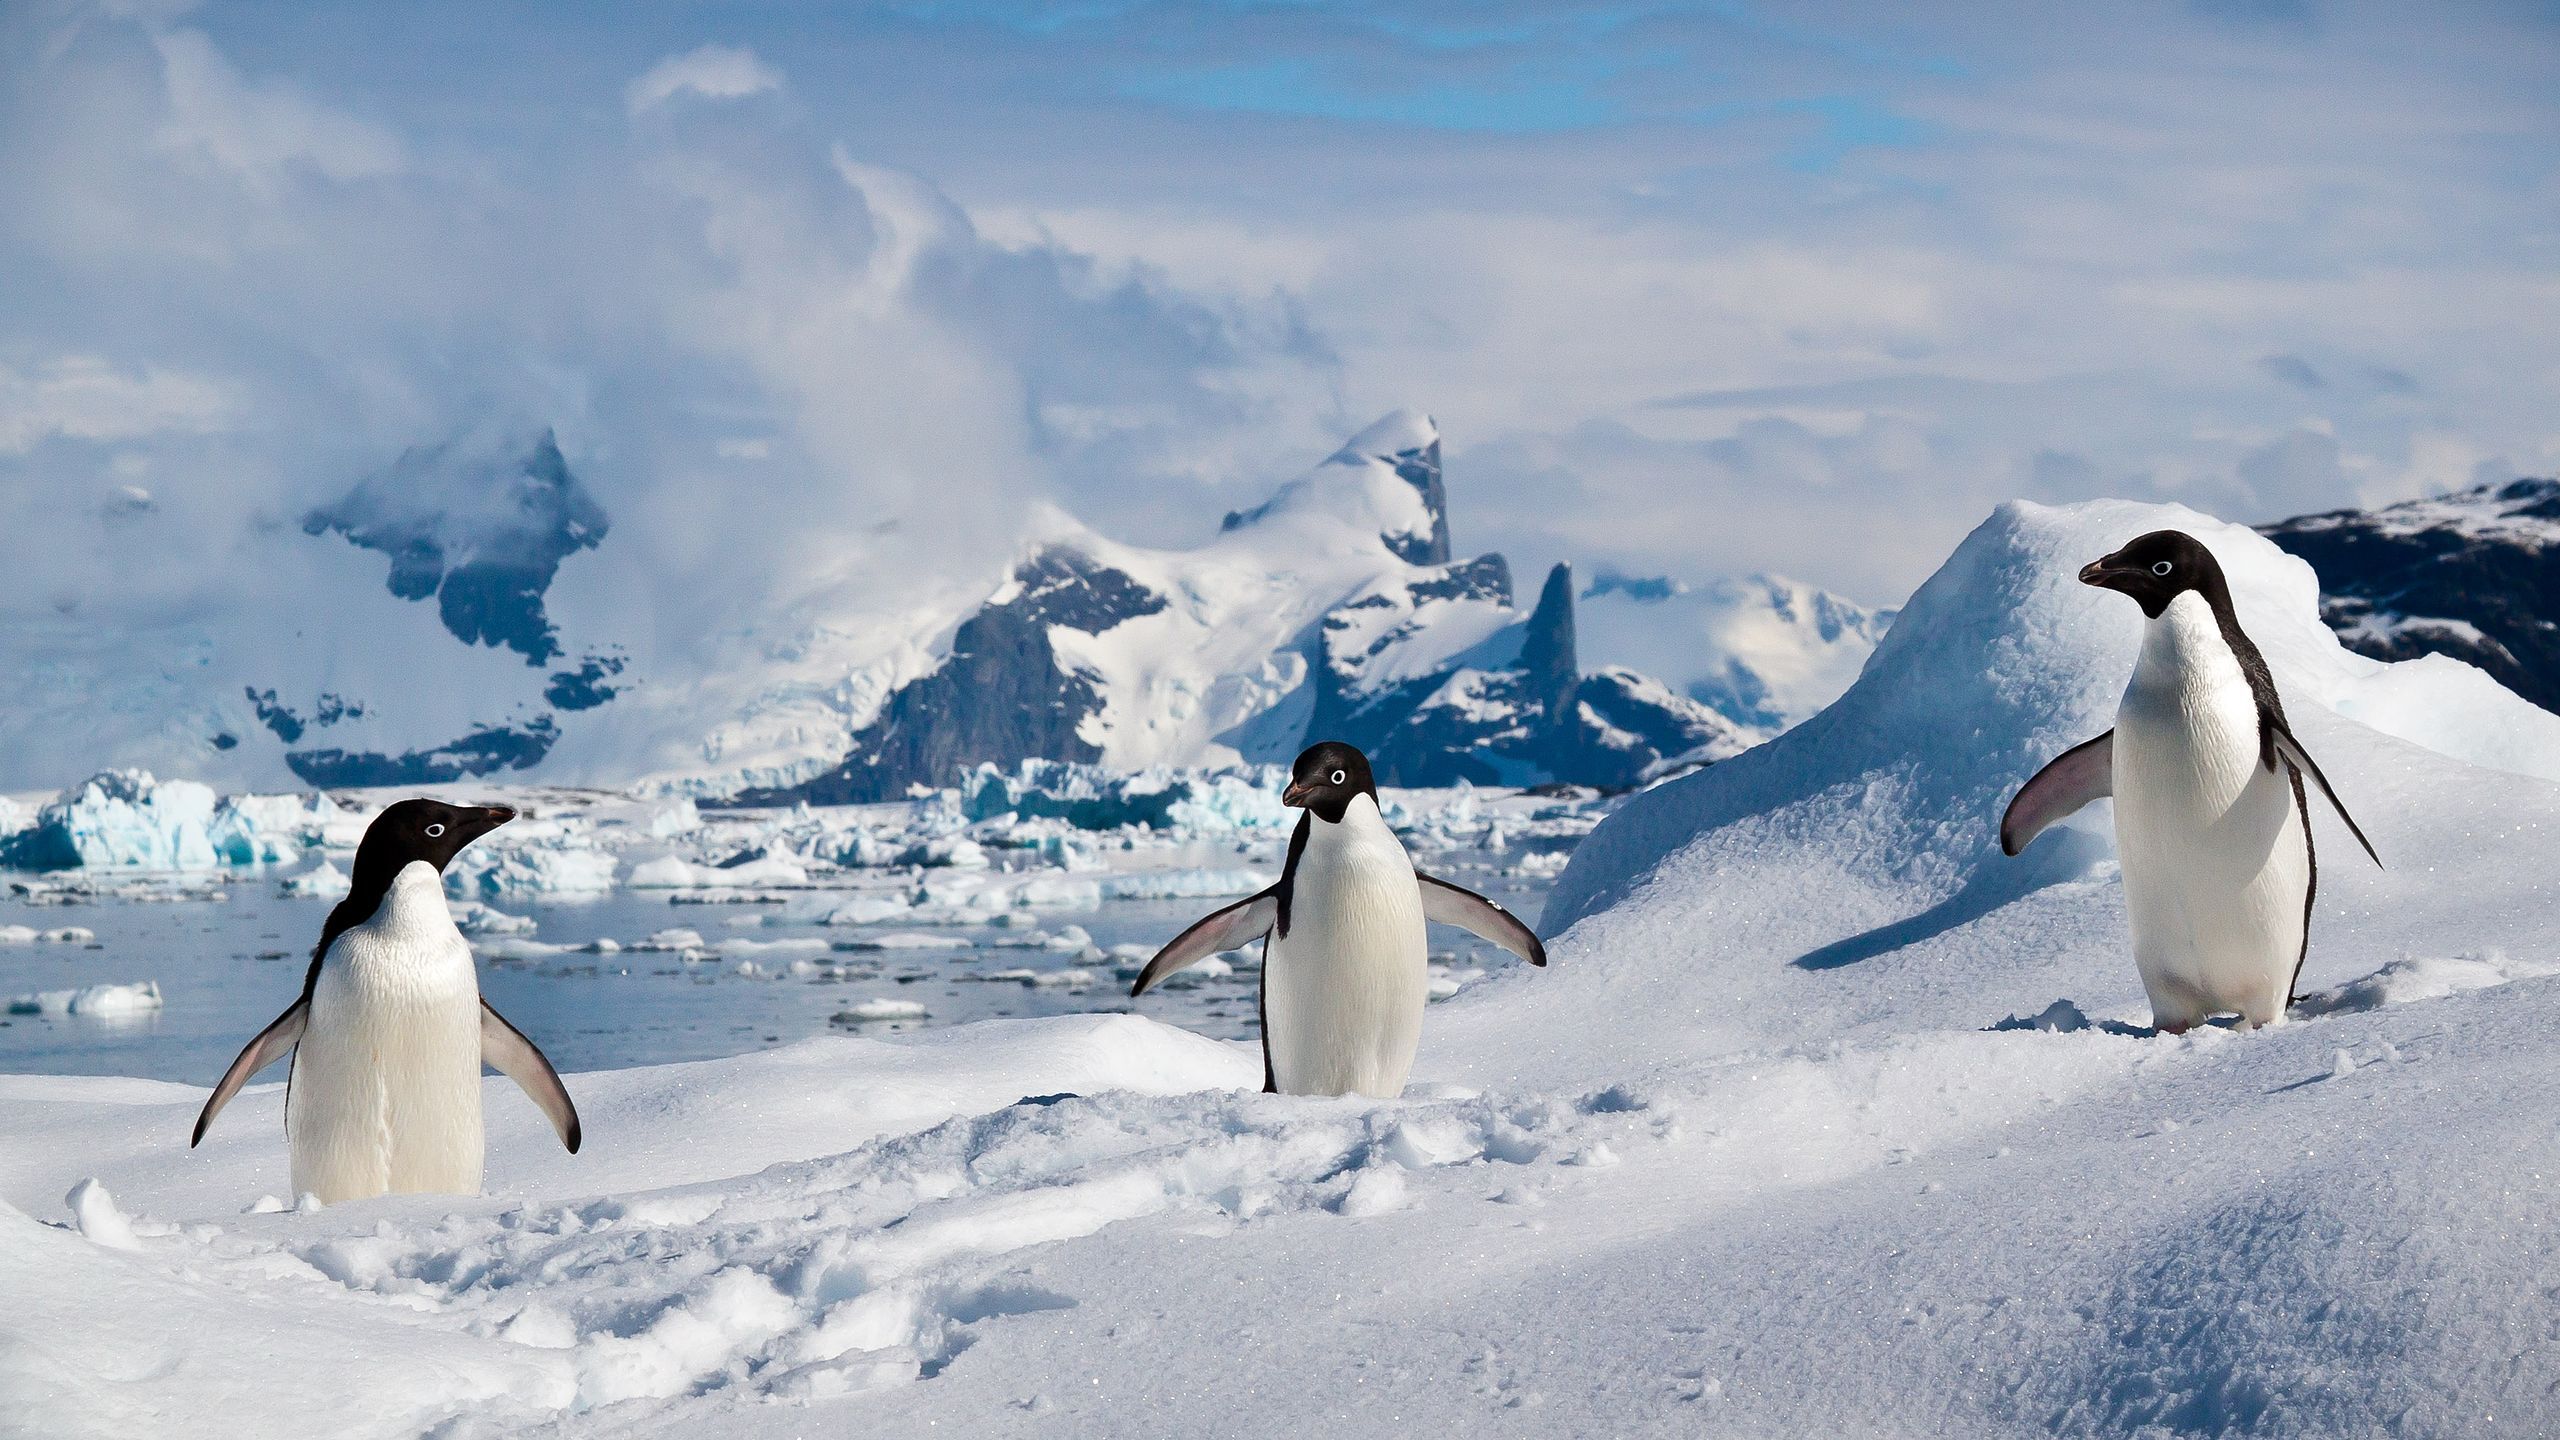
\includegraphics[scale=0.1]{Adelie_penguins_in_the_South_Shetland_Islands.jpg}
    \caption{Scaling it down}
    \label{fig:adelie_penguins_scaled}
\end{figure}

		
\end{document}